\documentclass[b5paper,xelatex,ja=standard,11pt]{bxjsarticle}

% 余白を詰めてページ番号を下げる設定
\setpagelayout*{
  top=13truemm,
  bottom=18truemm,
  left=15truemm,
  right=15truemm}
\addtolength{\footskip}{5mm}

% 行間をやや詰める設定
\usepackage{leading}
\leading{14.5pt}
\usepackage{setspace}  % 目次の行間を詰める用

% 色名の読み込みと独自色定義
\usepackage[x11names]{xcolor}
\definecolor{TextColor}{RGB}{51,51,51}  % #333333
\definecolor{PaleIris}{RGB}{229,227,246}
\definecolor{PaleGold}{RGB}{255,247,204}
\definecolor{PaleIris2}{RGB}{173,165,223}
\definecolor{PaleGold2}{RGB}{248,222,75}

% 数式フォント用
\usepackage[mathrm=sym]{unicode-math}
\usepackage{amsmath}

% フォント定義 (日本語は小さめにスケール)
% 等幅フォントにはシンタクスハイライトを適用するために色を設定しない
% その代わりコード入りカラーボックスはページをまたげない
\setmainfont[Color=TextColor, BoldFont={MPLUS1-ExtraBold.ttf},]{MPLUS1-Regular.ttf}
\setCJKmainfont[Scale=0.95, Color=TextColor, BoldFont={MPLUS1-ExtraBold.ttf}]{MPLUS1-Regular.ttf}
\setCJKsansfont[Scale=0.95, Color=TextColor]{MPLUS1-ExtraBold.ttf}
\setsansfont[Color=TextColor]{MPLUS1-ExtraBold.ttf}
\setmonofont[Scale=1.0]{MPLUS1Code-Regular.ttf}  % 等幅
\setCJKmonofont[Scale=0.95]{MPLUS1Code-Regular.ttf}  % 日本語等幅

% 目次に点線を引く設定
\makeatletter
\renewcommand*\l@section{\@dottedtocline{1}{0.0em}{4.0em}}
\makeatother

% ソースコード表示設定
\usepackage{listings}
\usepackage[most,listings]{tcolorbox}
\tcbuselibrary{breakable}
\lstset{  % グローバル設定
  columns=fixed,  % 等幅
  basewidth=0.5em,  % 字間詰め
  lineskip=-3pt,  % 行間詰め
  basicstyle={\ttfamily\color{TextColor}},  % 全体フォント設定
  keywordstyle=[1]{\color{DodgerBlue3}},  % kewords[1]の設定 (Python だと予約語)
  keywordstyle=[2]{\color{VioletRed3}},  % kewords[2]の設定 (Python だと組み込み関数)
  stringstyle={\color{Firebrick3}},  % 文字列リテラルの設定
  commentstyle={\color{SeaGreen4}},  % コメントの設定
  showstringspaces=false,  % 半角スペース記号を表示しない (コピペの邪魔)
}

% 独自のセリフ用カラーボックスの定義
% 共通設定
\tcbset{
  serifubox/.style={
    enhanced,  % タイトルボックスの表示に必要
    breakable,  % ページをまたぐのに必要
    arc=7pt, top=7pt, right=7pt, left=7pt, bottom=7pt,  % パディング
    boxrule=0pt, frame hidden,  % フレーム隠蔽
    grow to left by=-31pt,  % キャラクター画像を表示するため左にマージン
    enlarge bottom by=-1pt, title={\,},
    attach boxed title to top left={xshift=-34pt, yshift=-40pt},
    boxed title style={
      enhanced, arc=19pt, top=17pt, right=15pt, left=17pt, bottom=17pt,
      boxrule=0pt, frame hidden, underlay={\begin{tcbclipinterior}
        \includegraphics[width=39pt,keepaspectratio]{#1}\end{tcbclipinterior}},
    }
  }
}
% 部長
\newtcolorbox{SERIFU1}[1][]{
  serifubox={../images/a0_.png},
  colback=PaleIris, colbacktitle=PaleIris2, #1
}
% 副部長
\newtcolorbox{SERIFU2}[1][]{
  serifubox={../images/b0_.png},
  colback=PaleGold, colbacktitle=PaleGold2, #1
}

% 独自の汎用カラーボックスの定義
% 共通設定
\tcbset{
  custombox/.style={
    enhanced,  % タイトルボックスの表示に必要
    breakable,  % ページをまたぐのに必要
    arc=2pt, colframe=TextColor, boxrule=1pt, colback=Snow1,
    right=7pt, left=7pt,
    title={\addfontfeatures{Color=white}\addCJKfontfeatures{Color=white}\textbf{#1}}
  }
}
% 独自のコード用カラーボックスの定義
\newtcolorbox{CODE}[2][]{
  custombox={#2}, top=0pt, bottom=0pt, #1
}
% 独自の命題枠の定義
\newtcolorbox{PROP}[2][]{
  custombox={#2}, top=7pt, bottom=7pt, #1
}

\usepackage{eso-pic}
% 表紙背景を cover.png で埋め尽くしたいときは以下
% \newcommand\BackgroundPic{\put(-0.01\paperwidth, -0.01\paperheight){%
% \parbox[b][\paperheight]{\paperwidth}{\vfill\centering
% \includegraphics[width=1.02\paperwidth, keepaspectratio]{cover.png}\vfill}}}
\usepackage{pagecolor}  % 表紙背景を無地で塗りつぶすときに使う

% 奥付
\newtcolorbox{OKUDUKE}[1][]{
  enhanced, sharp corners, colbacktitle=white, colback=white, colframe=TextColor,
  toprule=1.5pt, bottomrule=1.5pt, rightrule=0pt, leftrule=0pt,
  segmentation style={TextColor, dotted, line width=1pt},
  top=4pt, right=2pt, left=2pt, bottom=2pt, middle=3pt,  % パディング
  grow to left by=-20pt, grow to right by=-20pt,  % マージン
  attach boxed title to top left={yshift=3pt},
  boxed title style={skin=enhancedfirst jigsaw, boxrule=0pt, frame hidden, top=0pt},
  #1
}

% ハイパーリンク
\PassOptionsToPackage{hyphens}{url}
\usepackage[colorlinks=true]{hyperref}
\hypersetup{urlcolor=SteelBlue3}

% ======================================================================
\begin{document}

\definecolor{CoverBackColor}{RGB}{153,196,214}
\definecolor{CoverColor}{RGB}{234,239,242}
\newfontfamily{\mpblacke}[Color=TextColor]{MPLUS1-Black.ttf}
\newCJKfontfamily{\mpblack}[Color=TextColor]{MPLUS1-Black.ttf}
\newCJKfontfamily{\mpblackc}[Color=CoverColor]{MPLUS1-Black.ttf}
\pagecolor{CoverBackColor}
\setlength{\fboxsep}{7pt}
\newcommand*{\mybooktitle}{ニューラルネットによる時系列予測の話}

% タイトルページ
\AddToShipoutPicture*{
% \BackgroundPic  % 表紙背景を cover.png で埋め尽くす場合
% タイトル記述
\AtPageCenter{\put(-0.43\textwidth, 0.2\textheight){\parbox{.86\textwidth}{%
{\mpblacke\fontsize{18pt}{10pt}\selectfont A Small Talk about Neural Networks
for Time Series Forecasting \rule[-0.4em]{0pt}{1.3em}} \\
{\mpblackc\fontsize{42pt}{5pt}\selectfont
\colorbox{TextColor}{ニューラルネット} \vspace{-12pt} \\
\colorbox{TextColor}{による時系列予測} \vspace{-12pt} \\
\colorbox{TextColor}{の話}
\rule[-0.5em]{0pt}{0pt}} \\
{\mpblack\fontsize{30pt}{10pt}\selectfont クッキー}
}}}
% バージョン記述
\AtPageCenter{\put(-0.43\textwidth, -0.415\textheight){\parbox{.86\textwidth}{%
{\mpblacke\fontsize{27pt}{10pt}\selectfont Ver}
\raisebox{0.1em}{\mpblack\fontsize{25pt}{10pt}\selectfont 技術書典}
{\mpblacke\fontsize{27pt}{10pt}\selectfont 16}
}}}
% イラスト挿入
\AtPageCenter{\put(0.03\textwidth, -0.45\textheight){
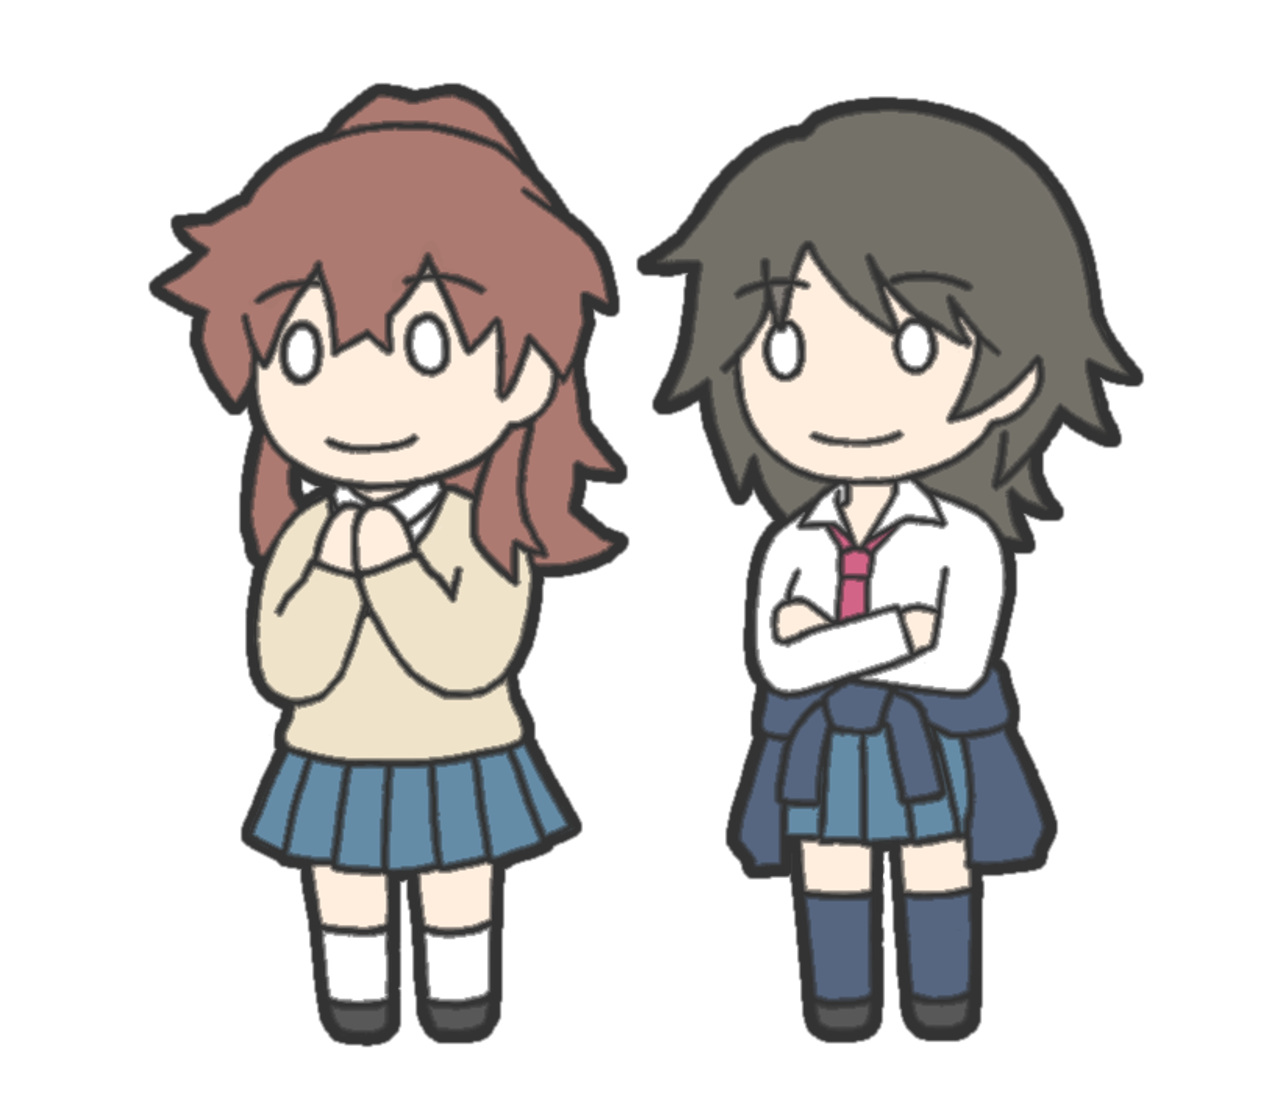
\includegraphics[width=0.44\textwidth]{../images/ab.png}
}}
}

\begin{titlepage}
\ 
\end{titlepage}
\pagecolor{none}

\newcommand*{\mysectiontitle}{まえがき}
\section*{\mysectiontitle}
% \addcontentsline{toc}{section}{\mysectiontitle}  % まえがきを目次に登録するか

本書の内容についてお気付きの点がありましたら、
大変お手数ですが、この本の原稿リポジトリの
 Issues \footnote{\url{https://github.com/CookieBox26/notes-2024/issues}}
または著者メール \footnote{cookie-box[at]cookie-box.info} までご連絡ください。

\addcontentsline{toc}{section}{参考文献}
\begin{thebibliography}{9}
  \bibitem{bib1} 参考文献。
\end{thebibliography}

\vspace{7pt}\centerline{\large\bf 登場人物紹介}
\vspace{-20pt}
\noindent
\begin{minipage}[t]{0.33\textwidth}
\centering
\strut\vspace*{-\baselineskip}
\newline\newline
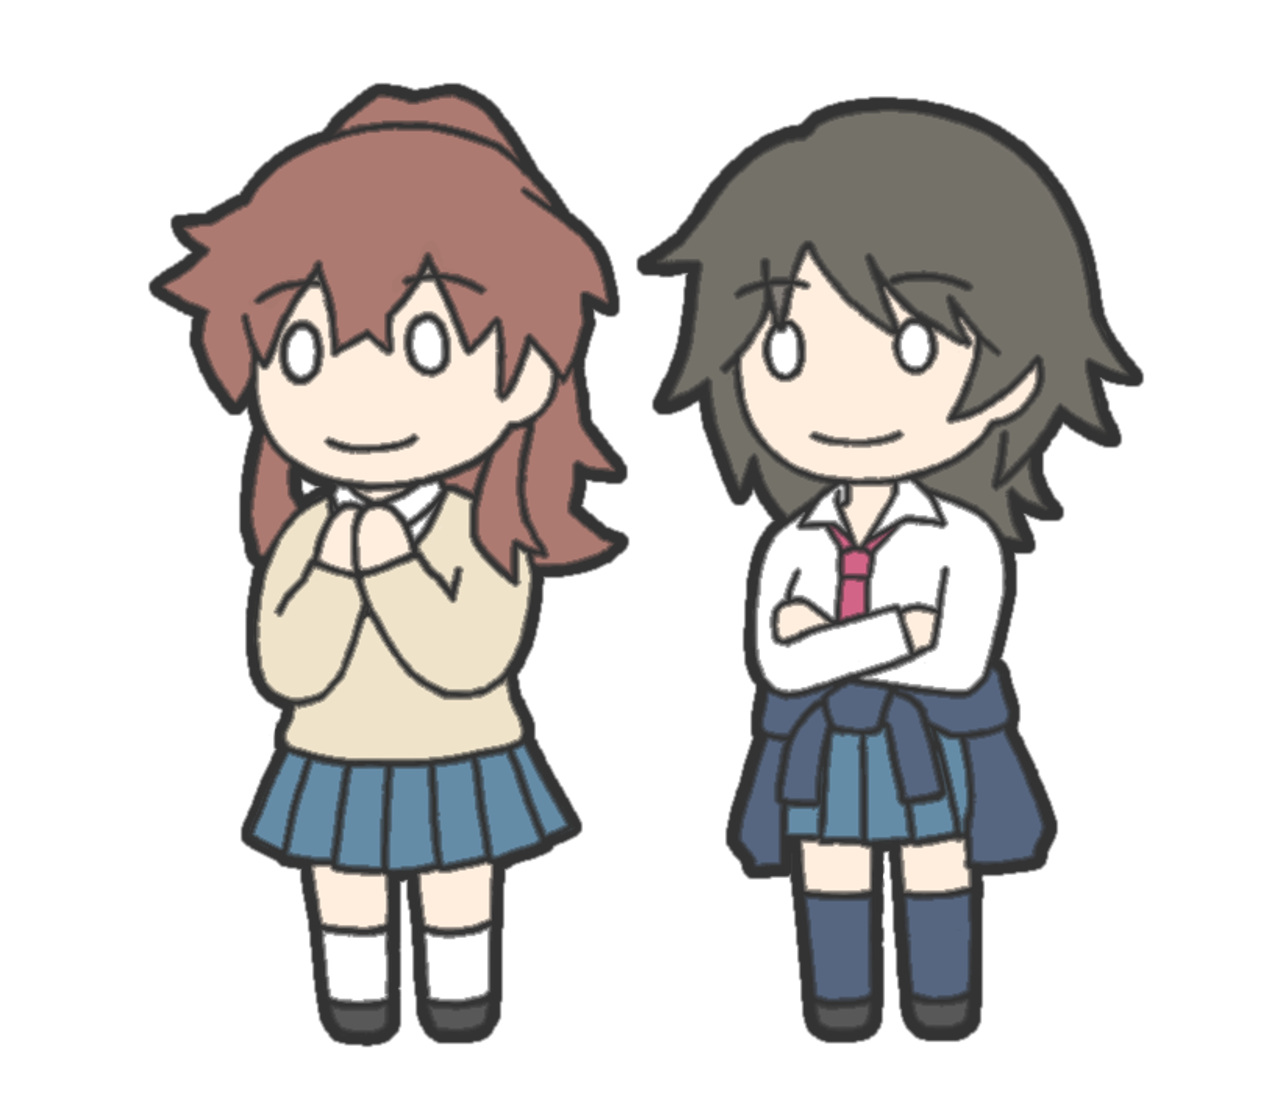
\includegraphics[width=1.0\textwidth,keepaspectratio]{../images/ab.png}
\end{minipage}
\begin{minipage}[t]{0.67\textwidth}
\vspace{18pt}
 左側の人は部長です。1年生です。
統計や機械学習を学ぶ部活動を立ち上げ、勉強しています。\\
 右側の人は副部長です。海外から編入してきた2年生で、
部長に勧誘されて部に入部しました。\\
 部には部長と副部長しかいません。\\
 これらの設定は本編と関係ありません。
\end{minipage}

\begin{spacing}{1.1}\textbf{\tableofcontents}\end{spacing}

\newcounter{mycounter}
\stepcounter{mycounter}
\renewcommand*{\mysectiontitle}{第{\themycounter}話 \, ほげほげ}
\section*{\mysectiontitle}\addcontentsline{toc}{section}{\mysectiontitle}

\begin{SERIFU1}[enlarge top by=3pt]
こんにちは Hello こんにちは{\bf こんにちは}こんにちはこんにちは
こんにちはこんにちはこんにちはこんにちはこんにちはこんにちは。
\end{SERIFU1}

\begin{SERIFU2}
こんにちは Hello こんにちは{\bf こんにちは}こんにちはこんにちは
こんにちはこんにちはこんにちはこんにちはこんにちはこんにちは。
\end{SERIFU2}

\begin{SERIFU1}
こんにちは Hello こんにちは{\bf こんにちは}こんにちはこんにちは
こんにちはこんにちはこんにちはこんにちはこんにちはこんにちは。
こんにちは Hello こんにちは{\bf こんにちは}こんにちはこんにちは
こんにちはこんにちはこんにちはこんにちはこんにちはこんにちは。
\end{SERIFU1}

\begin{SERIFU2}[enlarge bottom by=2pt]
こんにちは Hello こんにちは{\bf こんにちは}こんにちはこんにちは
こんにちはこんにちはこんにちはこんにちはこんにちはこんにちは。
\end{SERIFU2}

こんにちは Hello こんにちは{\bf こんにちは}こんにちはこんにちは
こんにちはこんにちはこんにちはこんにちはこんにちはこんにちは。

\begin{CODE}{Pythonスクリプト}
\begin{lstlisting}[language=python]
import numpy as np
import pandas as pd
%matplotlib inline  
import matplotlib.pyplot as plt
import matplotlib.patches as patches
from matplotlib.colors import to_rgba
from matplotlib import font_manager
plt.rcParams['font.family'] = 'Ume Gothic'
plt.rcParams['font.size'] = 12
plt.rcParams['axes.linewidth'] = 1.5
plt.rcParams['grid.linewidth'] = 1.5
print(type(123))  # コメント
\end{lstlisting}
\end{CODE}

\stepcounter{mycounter}
\renewcommand*{\mysectiontitle}{第{\themycounter}話 \, ふがふが}
\section*{\mysectiontitle}\addcontentsline{toc}{section}{\mysectiontitle}

\begin{SERIFU1}[enlarge top by=3pt]
こんにちは Hello こんにちは{\bf こんにちは}こんにちはこんにちは
こんにちはこんにちはこんにちはこんにちはこんにちはこんにちは。
\end{SERIFU1}

\begin{SERIFU2}
こんにちは Hello こんにちは{\bf こんにちは}こんにちはこんにちは
こんにちはこんにちはこんにちはこんにちはこんにちはこんにちは。
\end{SERIFU2}

\begin{SERIFU1}
こんにちは Hello こんにちは{\bf こんにちは}こんにちはこんにちは
こんにちはこんにちはこんにちはこんにちはこんにちはこんにちは。
\end{SERIFU1}

\begin{SERIFU2}[enlarge bottom by=5pt]
こんにちは Hello こんにちは{\bf こんにちは}こんにちはこんにちは
こんにちはこんにちはこんにちはこんにちはこんにちはこんにちは。
\end{SERIFU2}

\begin{PROP}{定理 0.1.0 〈\, 制約がないときの1次の必要条件 \,〉}
$x^\ast$ を問題(P)の局所最適解とする。但し、$f$ は $x^\ast$ で微分可能であるものとする。
 (P) $\displaystyle \underset{x \in \mathbb{R}^n}{\mathrm{minimize}} \; \; f(x)$
このとき,以下を満たす $s \in \mathbb{R}^n$ は存在しない。
\begin{eqnarray*}
\nabla f(x^\ast)^\top s < 0
\end{eqnarray*}
\end{PROP}

\rightline{\large\bf 終わり}

% 奥付
\clearpage
\vspace*{0.75\textheight}
\begin{OKUDUKE}[title={\large\bf \mybooktitle}]
2024年5月25日 初版発行
\tcblower
\renewcommand\arraystretch{0.95}
\begin{tabular}{rp{10cm}}
著 者 & クッキー \\
発行者 & クッキーの日記 \\
& \url{https://cookie-box.hatenablog.com/} 
\end{tabular}
\end{OKUDUKE}
\thispagestyle{empty}

\end{document}
% ======================================================================
